\subsection{Area 2 – Docenti}
\begin{figure}[H]
\centering
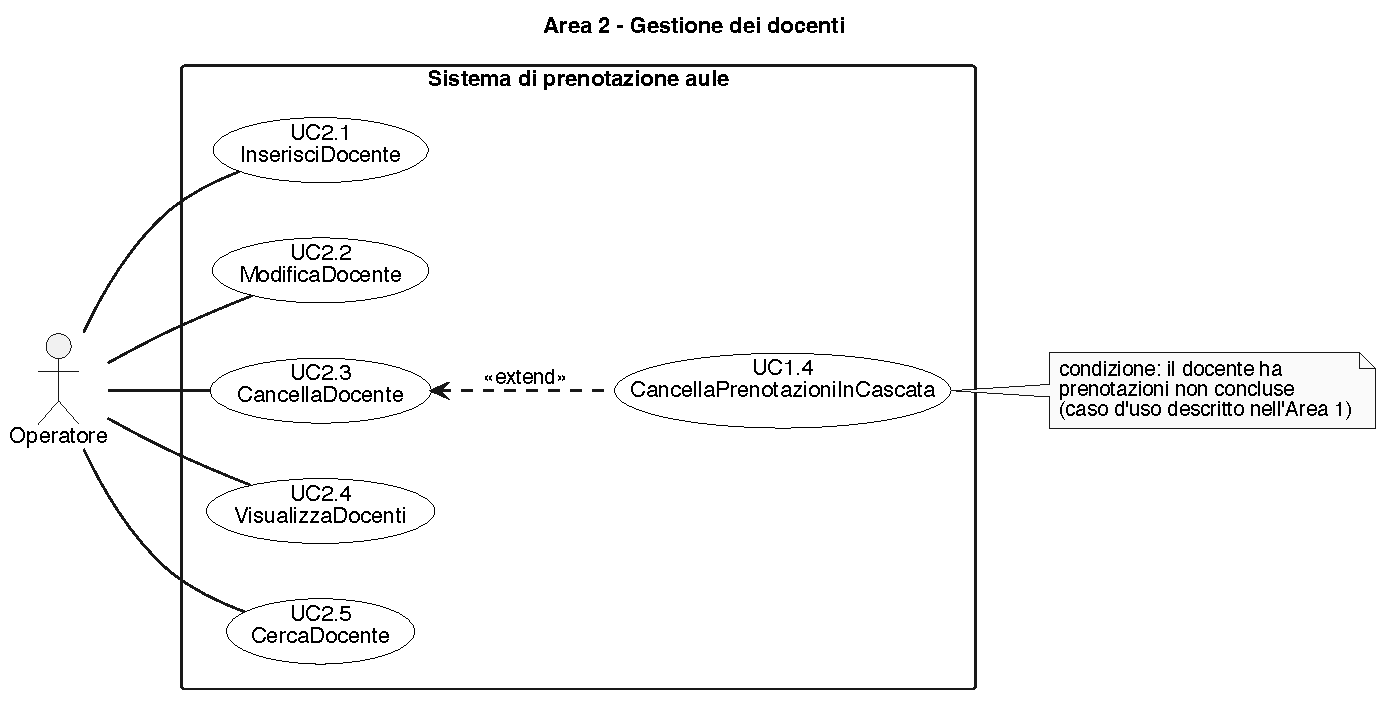
\includegraphics[width=\textwidth,height=0.8\textheight,keepaspectratio]{diagrammi/uc-area2-docenti}
\caption{Casi d'uso dell'Area 2 – Docenti}
\end{figure}

\subsubsection{[UC2.1] InserisciDocente}
\noindent Attore: Operatore\\
Requisiti correlati: FI2.1, ED2.1–ED2.3, IU2.1, IU2.2, IU4.6, IU4.7\\
Pre-condizioni: Il sistema mostra la sezione Docenti.\\
Post-condizioni: Il nuovo docente è registrato nell'archivio, l'archivio è salvato su file e il docente compare nella lista dei docenti.\\

\noindent Flusso principale:
\begin{enumerate}
\item L'Operatore sceglie il comando Nuovo docente.
\item Il sistema mostra il modulo del docente con i campi e-mail, nome e cognome vuoti.
\item L'Operatore compila i campi e conferma.
\item Il sistema verifica che i dati rispettino i vincoli ED2.1 ed ED2.3.
\item Il sistema verifica che non esista un altro docente con la stessa e-mail (ED2.2).
\item Il sistema registra il docente, salva l'archivio, chiude il modulo e mostra la lista aggiornata con un messaggio di esito.
\end{enumerate}
\noindent Flussi alternativi:
\begin{itemize}
\item \textbf{3a.} L'Operatore annulla: si applica FC1.
\item \textbf{4a.} Uno o più dati non sono validi (es. campo vuoto, e-mail non del dominio \texttt{unisa.it}):
\begin{itemize}
\item 4a.1 Il sistema indica ogni campo errato e il vincolo da rispettare;
\item 4a.2 si riprende dal passo 3.
\end{itemize}
\item \textbf{5a.} Esiste già un docente con la stessa e-mail:
\begin{itemize}
\item 5a.1 Il sistema segnala che l'e-mail è già registrata;
\item 5a.2 si riprende dal passo 3.
\end{itemize}
\item \textbf{6a.} Il salvataggio non riesce: si applica FC2.
\end{itemize}

\subsubsection{[UC2.2] ModificaDocente}
\noindent Attore: Operatore\\
Requisiti correlati: FI2.2, ED2.1, IU2.1, IU2.2, IU4.6, IU4.7\\
Pre-condizioni: Il sistema mostra la sezione Docenti e nell'archivio è registrato almeno un docente.\\
Post-condizioni: Nome e cognome del docente sono aggiornati nell'archivio, l'archivio è salvato su file e la lista mostra i nuovi valori nel corretto ordine. E-mail e prenotazioni del docente non cambiano.\\

\noindent Flusso principale:
\begin{enumerate}
\item L'Operatore seleziona un docente nella lista (o tra i risultati di una ricerca) e sceglie il comando Modifica.
\item Il sistema mostra il modulo del docente con i dati attuali; l'e-mail è visibile ma non modificabile.
\item L'Operatore modifica nome e/o cognome e conferma.
\item Il sistema verifica che i dati rispettino il vincolo ED2.1.
\item Il sistema aggiorna il docente, salva l'archivio, chiude il modulo e mostra la lista aggiornata con un messaggio di esito.
\end{enumerate}
\noindent Flussi alternativi:
\begin{itemize}
\item \textbf{1a.} L'Operatore sceglie Modifica senza aver selezionato un docente:
\begin{itemize}
\item 1a.1 Il sistema chiede di selezionare un docente;
\item 1a.2 si riprende dal passo 1.
\end{itemize}
\item \textbf{3a.} L'Operatore annulla: si applica FC1.
\item \textbf{4a.} Uno o più dati non sono validi:
\begin{itemize}
\item 4a.1 Il sistema indica ogni campo errato e il vincolo da rispettare;
\item 4a.2 si riprende dal passo 3.
\end{itemize}
\item \textbf{5a.} Il salvataggio non riesce: si applica FC2.
\end{itemize}

\subsubsection{[UC2.3] CancellaDocente}
\noindent Attore: Operatore\\
Requisiti correlati: FI2.3, FI2.4, IU4.3, IU4.7, NF7\\
Pre-condizioni: Il sistema mostra la sezione Docenti e nell'archivio è registrato almeno un docente.\\
Post-condizioni: Il docente e le sue prenotazioni concluse sono rimossi dall'archivio, l'archivio è salvato su file e il docente non compare più nella lista.\\
Punto di estensione: Passo 2: il docente ha prenotazioni non concluse $\rightarrow$ UC1.4 CancellaPrenotazioniInCascata.\\

\noindent Flusso principale:
\begin{enumerate}
\item L'Operatore seleziona un docente nella lista e sceglie il comando Cancella.
\item Il sistema verifica che il docente non abbia prenotazioni non concluse.
\item Il sistema chiede conferma mostrando i dati del docente (IU4.3).
\item L'Operatore conferma.
\item Il sistema rimuove il docente e le sue eventuali prenotazioni concluse, salva l'archivio e mostra la lista aggiornata con un messaggio di esito.
\end{enumerate}
\noindent Flussi alternativi:
\begin{itemize}
\item \textbf{1a.} L'Operatore sceglie Cancella senza aver selezionato un docente:
\begin{itemize}
\item 1a.1 Il sistema chiede di selezionare un docente;
\item 1a.2 si riprende dal passo 1.
\end{itemize}
\item \textbf{2a.} Il docente ha almeno una prenotazione non conclusa:
\begin{itemize}
\item 2a.1 si esegue UC1.4 CancellaPrenotazioniInCascata e il caso d'uso termina.
\end{itemize}
\item \textbf{4a.} L'Operatore annulla: si applica FC1.
\item \textbf{5a.} Il salvataggio non riesce: si applica FC2.
\end{itemize}

\subsubsection{[UC2.4] VisualizzaDocenti}
\noindent Attore: Operatore\\
Requisiti correlati: FI2.5, IU2.1, IU4.1\\
Pre-condizioni: Nessuna oltre alla precondizione comune.\\
Post-condizioni: Il sistema mostra tutti i docenti registrati ordinati per cognome e nome. L'archivio è invariato.\\

\noindent Flusso principale:
\begin{enumerate}
\item L'Operatore apre la sezione Docenti.
\item Il sistema mostra la tabella di tutti i docenti registrati, con cognome, nome ed e-mail, ordinati per cognome, poi per nome, poi per e-mail (FI2.5).
\end{enumerate}
\noindent Flussi alternativi:
\begin{itemize}
\item \textbf{2a.} Non è registrato nessun docente:
\begin{itemize}
\item 2a.1 Il sistema mostra la tabella vuota con il messaggio ``Nessun docente registrato''.
\end{itemize}
\end{itemize}

\subsubsection{[UC2.5] CercaDocente}
\noindent Attore: Operatore\\
Requisiti correlati: FI2.6, FI2.7, IU2.1, IU4.6\\
Pre-condizioni: Il sistema mostra la sezione Docenti.\\
Post-condizioni: Il sistema mostra i docenti che soddisfano il criterio scelto, ordinati come in FI2.5. L'archivio è invariato.\\

\noindent Flusso principale:
\begin{enumerate}
\item L'Operatore sceglie il criterio di ricerca (cognome o e-mail) e inserisce il valore.
\item L'Operatore avvia la ricerca.
\item Il sistema verifica che il valore non sia vuoto.
\item Il sistema mostra i docenti che soddisfano il criterio:
\begin{itemize}
\item per \textbf{cognome}: i docenti il cui cognome contiene il testo inserito, senza distinguere maiuscole e minuscole;
\item per \textbf{e-mail}: il docente con quell'e-mail, senza distinguere maiuscole e minuscole.
\end{itemize}
\end{enumerate}
\noindent Flussi alternativi:
\begin{itemize}
\item \textbf{3a.} Il valore è vuoto:
\begin{itemize}
\item 3a.1 Il sistema chiede di inserire un valore;
\item 3a.2 si riprende dal passo 1.
\end{itemize}
\item \textbf{4a.} Nessun docente soddisfa il criterio:
\begin{itemize}
\item 4a.1 Il sistema mostra la tabella vuota con il messaggio ``Nessun docente trovato''.
\end{itemize}
\item \textbf{4b.} L'Operatore sceglie di tornare alla lista completa:
\begin{itemize}
\item 4b.1 si esegue UC2.4 VisualizzaDocenti.
\end{itemize}
\end{itemize}
